\section{Overview}
\label{sec:overview}

QKD-Simulate is a program written in C++11 with a GUI based on the Qt library that simulates key generation according to the BB84 quantum key distribution scheme. The basic components of the system simulated by this program are shown in Figure \ref{fig:quantum_channel}.

\begin{figure}[h]
\centering
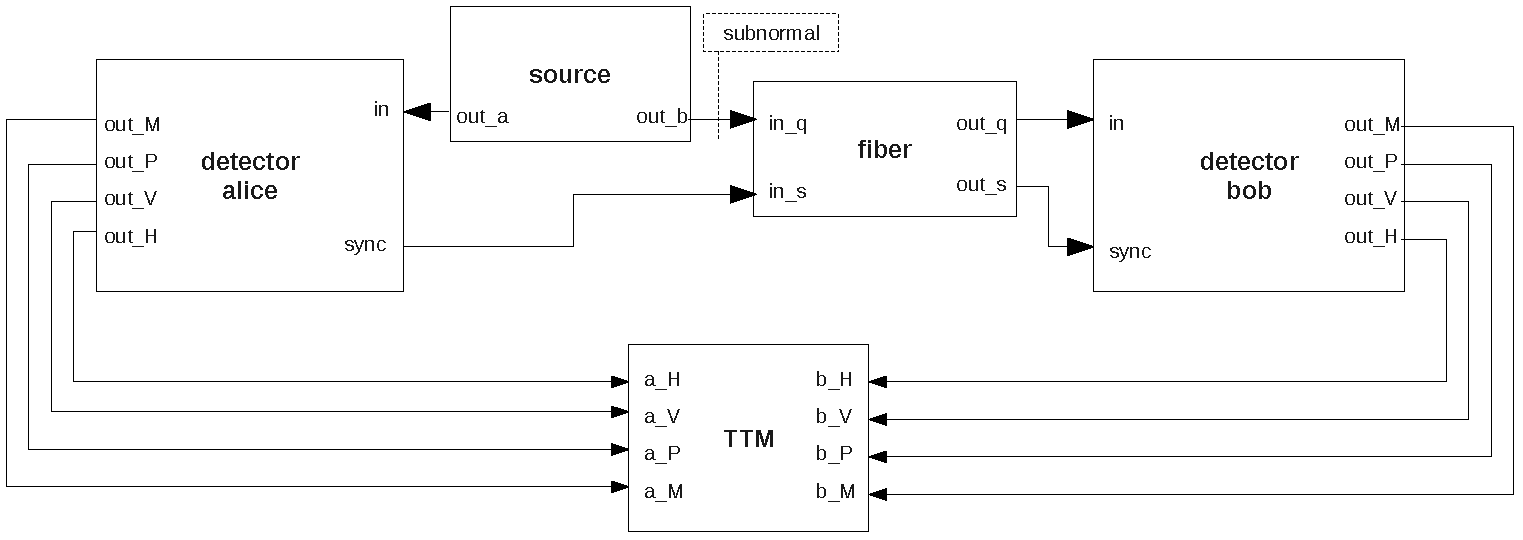
\includegraphics[scale=0.65]{drawings/channel.pdf}
\caption{The quantum key distribution system as modelled by the \texttt{channel} class}
\label{fig:quantum_channel}
\end{figure}

Actually, the components shown as rectangles with solid lines in this figure are instances of C++ classes that are defined in \texttt{.cpp} and \texttt{.h} files in the \texttt{channel} subdirectory of the \texttt{qkd-simulate} directory. Concretely, \textbf{source} is an instance of the \texttt{source} class defined in \texttt{source.h} and \texttt{source.cpp}, \textbf{fiber} is an instance of the \texttt{fiber} class defined in \texttt{fiber.h} and \texttt{fiber.cpp}, \textbf{TTM} is an instance of the \texttt{ttm} class defined in \texttt{ttm.h} and \texttt{ttm.cpp}, and \textbf{detector alice} and \textbf{detector bob} are two instances of the \texttt{detector} class defined in \texttt{detector.h} and \texttt{detector.cpp}, where a flag stored as a class member with name \texttt{m\_bAlice} of type \texttt{bool} is set to \texttt{true} for Alice's side and to \texttt{false} for Bob's side by a parameter named \texttt{bAlice} passed to the constructor at class instantiation. All of these class instances 
are contained in an instance of the \texttt{channel} class defined in \texttt{channel.h} and \texttt{channel.cpp} that manages the whole quantum key distribution simulation.
\\
\\
The physical process that should be simulated by this system is the following: The EPR (Einstein-Podolsky-Rosen) source creates pairs of entangled photons with a specific photon rate. For each created pair, one of the photons travels to the detector at Alice's side, the other one is transmitted over an optical fiber and travels to the detector at Bob's side. At first, the polarisation of the photon received by Alice's detector is measured in either the H/V (horizontal/vertical) or P/M (plus/minus) base (one of the two bases is selected randomly with equal probability\footnote{Changing this to unequal probabilities requires adaption of the \texttt{detector\_optics} class defined in \texttt{channel/detector/detector\_optics.h} and \texttt{channel/detector/detector\_optics.cpp}}) which causes a collapse of the entangled quantum state and determines the polarisation of the second photon (travelling to Bob's detector) which must be orthogonal to the polarisation state measured for the first photon by Alice's 
detector. Then, after some transmission delay time, the second photon is received by Bob's detector and its polarisation is measured in again either the H/V or the P/M basis chosen randomly. Alice's as well as Bob's detector contain four single-photon detection elements, one for each of the four possible photon polarisations.
\\
\\
What happens next depends on the system configuration:

\begin{itemize}

\item In the \textit{free running mode}, the single-photon detectors at Alice's and Bob's sides are enabled permanently, and for all received photons at Alice's or Bob's sides the TTM (Time Tagging Module) records the detection time and measured polarisation. In Figure \ref{fig:quantum_channel} only one TTM object is shown because in the C++ program, the \texttt{ttm} class is only instantiated once for simplicity, but in reality both Alice and Bob have their own TTM module.

\item In the \textit{sync mode} (for which also exist several variants that will be described later) the photon received by Alice's detector causes the generation of a sync pulse that is also transmitted over the fiber, but at another wavelength using WDM (wavelength-division multiplexing). Only when Bob's detector receives the sync pulse, it enables its single-photon detectors for some time so that they are ready to receive the second photon, which comes to Bob's detector a bit later than the sync pulse because it also travels through a delay fiber (not shown in Figure \ref{fig:quantum_channel}). The electrical pulses coming out of the single-photon detectors at Alice's and Bob's sides during some time window are then used for generating a binary string (4 bits each time a sync pulse is sent/received) that is stored in a buffer.

\end{itemize}